%\documentclass[handout]{ximera}
\documentclass[nooutcomes]{ximera}

\usepackage{gensymb}
\usepackage{tabularx}
\usepackage{mdframed}
\usepackage{pdfpages}
%\usepackage{chngcntr}

\let\problem\relax
\let\endproblem\relax

\newcommand{\property}[2]{#1#2}




\newtheoremstyle{SlantTheorem}{\topsep}{\fill}%%% space between body and thm
 {\slshape}                      %%% Thm body font
 {}                              %%% Indent amount (empty = no indent)
 {\bfseries\sffamily}            %%% Thm head font
 {}                              %%% Punctuation after thm head
 {3ex}                           %%% Space after thm head
 {\thmname{#1}\thmnumber{ #2}\thmnote{ \bfseries(#3)}} %%% Thm head spec
\theoremstyle{SlantTheorem}
\newtheorem{problem}{Problem}[]

%\counterwithin*{problem}{section}



%%%%%%%%%%%%%%%%%%%%%%%%%%%%Jenny's code%%%%%%%%%%%%%%%%%%%%

%%% Solution environment
%\newenvironment{solution}{
%\ifhandout\setbox0\vbox\bgroup\else
%\begin{trivlist}\item[\hskip \labelsep\small\itshape\bfseries Solution\hspace{2ex}]
%\par\noindent\upshape\small
%\fi}
%{\ifhandout\egroup\else
%\end{trivlist}
%\fi}
%
%
%%% instructorIntro environment
%\ifhandout
%\newenvironment{instructorIntro}[1][false]%
%{%
%\def\givenatend{\boolean{#1}}\ifthenelse{\boolean{#1}}{\begin{trivlist}\item}{\setbox0\vbox\bgroup}{}
%}
%{%
%\ifthenelse{\givenatend}{\end{trivlist}}{\egroup}{}
%}
%\else
%\newenvironment{instructorIntro}[1][false]%
%{%
%  \ifthenelse{\boolean{#1}}{\begin{trivlist}\item[\hskip \labelsep\bfseries Instructor Notes:\hspace{2ex}]}
%{\begin{trivlist}\item[\hskip \labelsep\bfseries Instructor Notes:\hspace{2ex}]}
%{}
%}
%% %% line at the bottom} 
%{\end{trivlist}\par\addvspace{.5ex}\nobreak\noindent\hung} 
%\fi
%
%


\let\instructorNotes\relax
\let\endinstructorNotes\relax
%%% instructorNotes environment
\ifhandout
\newenvironment{instructorNotes}[1][false]%
{%
\def\givenatend{\boolean{#1}}\ifthenelse{\boolean{#1}}{\begin{trivlist}\item}{\setbox0\vbox\bgroup}{}
}
{%
\ifthenelse{\givenatend}{\end{trivlist}}{\egroup}{}
}
\else
\newenvironment{instructorNotes}[1][false]%
{%
  \ifthenelse{\boolean{#1}}{\begin{trivlist}\item[\hskip \labelsep\bfseries {\Large Instructor Notes: \\} \hspace{\textwidth} ]}
{\begin{trivlist}\item[\hskip \labelsep\bfseries {\Large Instructor Notes: \\} \hspace{\textwidth} ]}
{}
}
{\end{trivlist}}
\fi


%% Suggested Timing
\newcommand{\timing}[1]{{\bf Suggested Timing: \hspace{2ex}} #1}




\hypersetup{
    colorlinks=true,       % false: boxed links; true: colored links
    linkcolor=blue,          % color of internal links (change box color with linkbordercolor)
    citecolor=green,        % color of links to bibliography
    filecolor=magenta,      % color of file links
    urlcolor=cyan           % color of external links
}

\title{Trigonometry Checkup}
\author{Bart Snapp and Brad Findell}

\outcome{Learning outcome goes here.}

\begin{document}
\begin{abstract}
  We review trigonometry.
\end{abstract}
\maketitle

\begin{teachingnote}
This activity can be done either as part of similarity or as a preactivity for Circular Trigonometry.  Perhaps recommend a special office hour for this.  
\end{teachingnote}
This activity is intended to remind you of key ideas from high school trigonometry. 

\begin{problem}
What are the ratios of side lengths in a $45^\circ$-$45^\circ$-$90^\circ$ triangle?  Explain where the ratios come from, including why they work for any such triangle, no matter what size.  (Hint: Use the Pythagorean Theorem.)
\end{problem}

\vspace{0.1in}

\begin{problem}
What are the ratios of side lengths in a $30^\circ$-$60^\circ$-$90^\circ$ triangle?  Explain where those the come from.  (Hint: How might an equilateral triangle help.)
\end{problem}

\vspace{0.1in}

\begin{problem}
Consider the right triangle below with an angle of $\alpha$, sides of length $x$ and $y$, and hypotenuse of length $r$, as labeled.  
%$$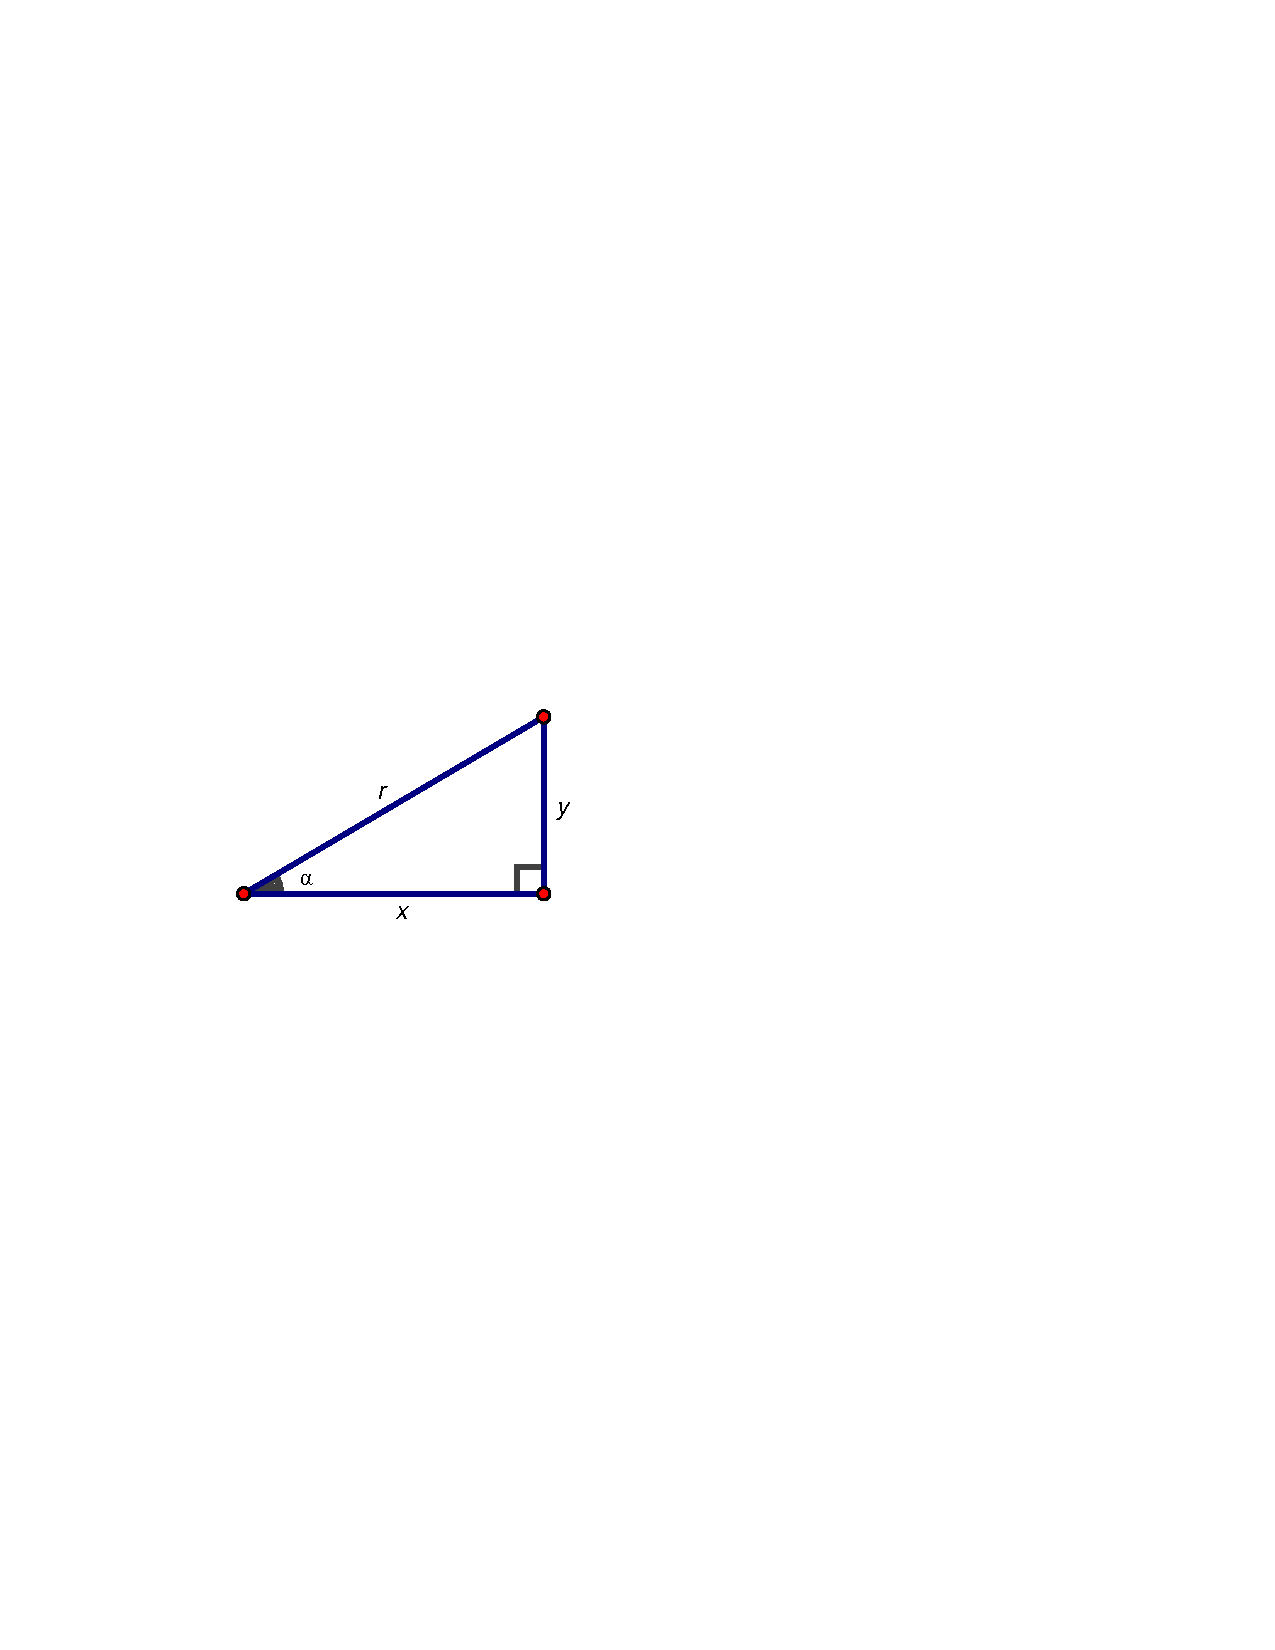
\includegraphics[scale=0.8]{../graphics/rightTriangle}$$
\[
\definecolor{qqwuqq}{rgb}{0.,0.392,0.}
\definecolor{qqqqff}{rgb}{0.,0.,1.}
\begin{tikzpicture}[line cap=round,line join=round,>=triangle 45,x=1.0cm,y=1.0cm]
\clip(-0.36,-0.34) rectangle (4.1,2.2);
\draw [shift={(0.,0.)},line width=0.8pt,color=qqwuqq,fill=qqwuqq,fill opacity=0.1] (0,0) -- (0.:0.5) arc (0.:29.745:0.5) -- cycle;
\draw [shift={(3.5,2.)},line width=0.8pt,color=qqwuqq,fill=qqwuqq,fill opacity=0.1] (0,0) -- (-150.26:0.5) arc (-150.26:-90.:0.5) -- cycle;
\draw[line width=0.8pt,color=qqwuqq,fill=qqwuqq,fill opacity=0.1] (3.5,0.28) -- (3.22,0.28) -- (3.22,0.) -- (3.5,0.) -- cycle; 
\draw [line width=0.8pt] (0.,0.)-- (3.5,2.);
\draw [line width=0.8pt] (3.5,2.)-- (3.5,0.);
\draw [line width=0.8pt] (3.5,0.)-- (0.,0.);
%\draw [fill=qqqqff] (0.,0.) circle (1.2pt);
%\draw [fill=qqqqff] (3.5,0.) circle (1.2pt);
%\draw [fill=qqqqff] (3.5,2.) circle (1.2pt);
\draw[color=qqwuqq] (0.85,0.2) node {$\alpha$};
%\draw[color=qqwuqq] (3.2,1.33) node {$\beta$};
\draw (1.8,-.2) node {$x$};
\draw (1.8,1.23) node {$r$};
\draw (3.7,1.) node {$y$};
\end{tikzpicture}
\]
\begin{enumerate}
\item If we imagine angle $\alpha$ is fixed, why are ratios of pairs of side lengths the same, no matter the size of the triangle?\margincomment{CCSS G-SRT.6. Understand that by similarity, side ratios in right triangles
  are properties of the angles in the triangle, leading to definitions
  of trigonometric ratios for acute angles.}
\vspace{0.3in}
\item Using the triangle above (and your memory of Precalculus), write down the side-length ratios for sine, cosine, and tangent:  
$$\sin\alpha = \hspace{1in} \cos\alpha = \hspace{1in} \tan\alpha =$$
\vspace{0.1in}
\item What values of $\alpha$ make sense in \emph{right triangle trigonometry}?  (We overcome these bounds later in circular trigonometry.)  
\vspace{0.3in}
\item What does it mean to say that these ratios depend upon the angle $\alpha$?  
\vspace{0.3in}
\item Why is only one of the triangle's three angles necessary in defining these ratios?  
\vspace{0.3in}
\end{enumerate}
\end{problem}

\begin{problem}
Use your work so far to find the following trigonometric ratios:
\begin{enumerate}
\itemsep 12pt
\item $\sin 30^\circ = \hspace{1in} \cos30^\circ = \hspace{1in} \tan30^\circ =$
\item $\sin 45^\circ = \hspace{1in} \cos45^\circ = \hspace{1in} \tan45^\circ =$
\item $\sin 60^\circ = \hspace{1in} \cos60^\circ = \hspace{1in} \tan60^\circ =$
\item $\sin 0^\circ = \hspace{1.08in} \cos0^\circ = \hspace{1.08in} \tan0^\circ =$
\end{enumerate}
\end{problem}

\vspace{0.2in}

\begin{problem}
You may recall the identity $\sin^2\theta+\cos^2\theta=1$.\margincomment{CCSS F-TF.8.  Prove the Pythagorean identity $\sin^2(\theta) + \cos^2(\theta) = 1$ and use it
  to find $\sin(\theta)$, $\cos(\theta)$, or $\tan(\theta)$ given $\sin(\theta)$, $\cos(\theta)$, or $\tan(\theta)$
  and the quadrant of the angle.}
\begin{enumerate}
\item Explain why the equation is true.  
\vspace{0.3in}
\item Why is it called an identity? 
\vspace{0.3in}
\item Why is it called a Pythagorean identity?  
\vspace{0.3in}
\end{enumerate}
\end{problem}

\begin{problem}
In right triangle trigonometry, there are indeed two acute angles, as shown in the figure below.\margincomment{CCSS G-SRT.7. Explain and use the relationship between the sine and cosine of
  complementary angles.}
%$$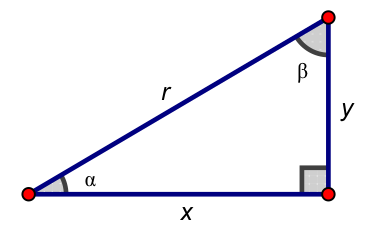
\includegraphics[scale=0.8]{../graphics/rightTriangle2}$$
\[
\definecolor{qqwuqq}{rgb}{0.,0.392,0.}
\definecolor{qqqqff}{rgb}{0.,0.,1.}
\begin{tikzpicture}[line cap=round,line join=round,>=triangle 45,x=1.0cm,y=1.0cm]
\clip(-0.36,-0.36) rectangle (4.1,2.2);
\draw [shift={(0.,0.)},line width=0.8pt,color=qqwuqq,fill=qqwuqq,fill opacity=0.1] (0,0) -- (0.:0.5) arc (0.:29.745:0.5) -- cycle;
\draw [shift={(3.5,2.)},line width=0.8pt,color=qqwuqq,fill=qqwuqq,fill opacity=0.1] (0,0) -- (-150.26:0.5) arc (-150.26:-90.:0.5) -- cycle;
\draw[line width=0.8pt,color=qqwuqq,fill=qqwuqq,fill opacity=0.1] (3.5,0.28) -- (3.22,0.28) -- (3.22,0.) -- (3.5,0.) -- cycle; 
\draw [line width=0.8pt] (0.,0.)-- (3.5,2.);
\draw [line width=0.8pt] (3.5,2.)-- (3.5,0.);
\draw [line width=0.8pt] (3.5,0.)-- (0.,0.);
%\draw [fill=qqqqff] (0.,0.) circle (1.2pt);
%\draw [fill=qqqqff] (3.5,0.) circle (1.2pt);
%\draw [fill=qqqqff] (3.5,2.) circle (1.2pt);
\draw[color=qqwuqq] (0.85,0.2) node {$\alpha$};
\draw[color=qqwuqq] (3.2,1.33) node {$\beta$};
\draw (1.8,-.2) node {$x$};
\draw (1.8,1.23) node {$r$};
\draw (3.7,1.) node {$y$};
\end{tikzpicture}
\]
\begin{enumerate}
\item How are the angles $\alpha$ and $\beta$ related?  Explain why.
\vspace{0.3in}
\item Using lengths in the above triangle, find the following ratios:    
$$\sin\alpha = \qquad\qquad\qquad \cos\alpha = $$
$$\sin\beta = \qquad\qquad\qquad \cos\beta = $$
\item What do you notice about the sine and cosine of complementary angles?  
\vspace{0.3in}
\item Explain why the result makes sense.  
\vspace{0.3in}
\end{enumerate}
\end{problem}

Given an angle and a side length of a right triangle, 
you can find the missing side lengths.\margincomment{CCSS G-SRT.8. Use trigonometric ratios and the Pythagorean Theorem to solve
  right triangles in applied problems.}
This is called ``solving the right triangle.''    And given the sine, cosine, or tangent of an angle, you can find the other two ratios.  (Hint: In either case, draw a triangle.)

%\begin{problem}
%A straight wire to the top of a flagpole meets the ground at a $25^\circ$ angle 30 feet from the base of the flag pole (on a flat lawn).  How high is the flagpole?  How long is the wire?  
%\end{problem}
%
%\vspace{0.5in}

\begin{problem}
Suppose $\sin\alpha = \frac{3}{5}$.  Then $\cos\alpha = \hspace{0.6in}$, $\tan\alpha = \hspace{0.6in}$.  
\end{problem}

\end{document}
